\chapter{Project Planning and Design}

\section{System Design}

\subsection{UML Diagrams}

UML, or Unified Modeling Language, is a standardized modeling language that consists of a set of diagrams used for modeling business processes and documenting software systems, helping better communicating potential designs and architectural decisions \parencite{uml}. 

The most common UML diagrams include:
\begin{itemize}
    \item \textbf{Use Case Diagram} - Illustrates the system's intended functionality in terms of actors, use cases, and their relationships, showing how the system delivers value to users.
    \item \textbf{Class Diagram} - Depicts the structure of the system by showing classes, attributes, operations, and static relationships between classes.
    \item \textbf{Sequence Diagram} - Demonstrates how objects interact in a particular, timed sequence scenario, focusing on the messages passed between objects.
    \item \textbf{Activity Diagram} - Represents the workflow of a target use case or business process through a series of activities, emphasizing steps, choices, iterations, and concurrency.
\end{itemize}

The student has used UML diagrams to present the stakeholders with a visual representation of the system's design and architecture. The diagrams can be found below.

\clearpage

\subsubsection{Use Case Diagram}

\begin{figure}[ht]
\label{fig:uml_usecase}
    \centering
    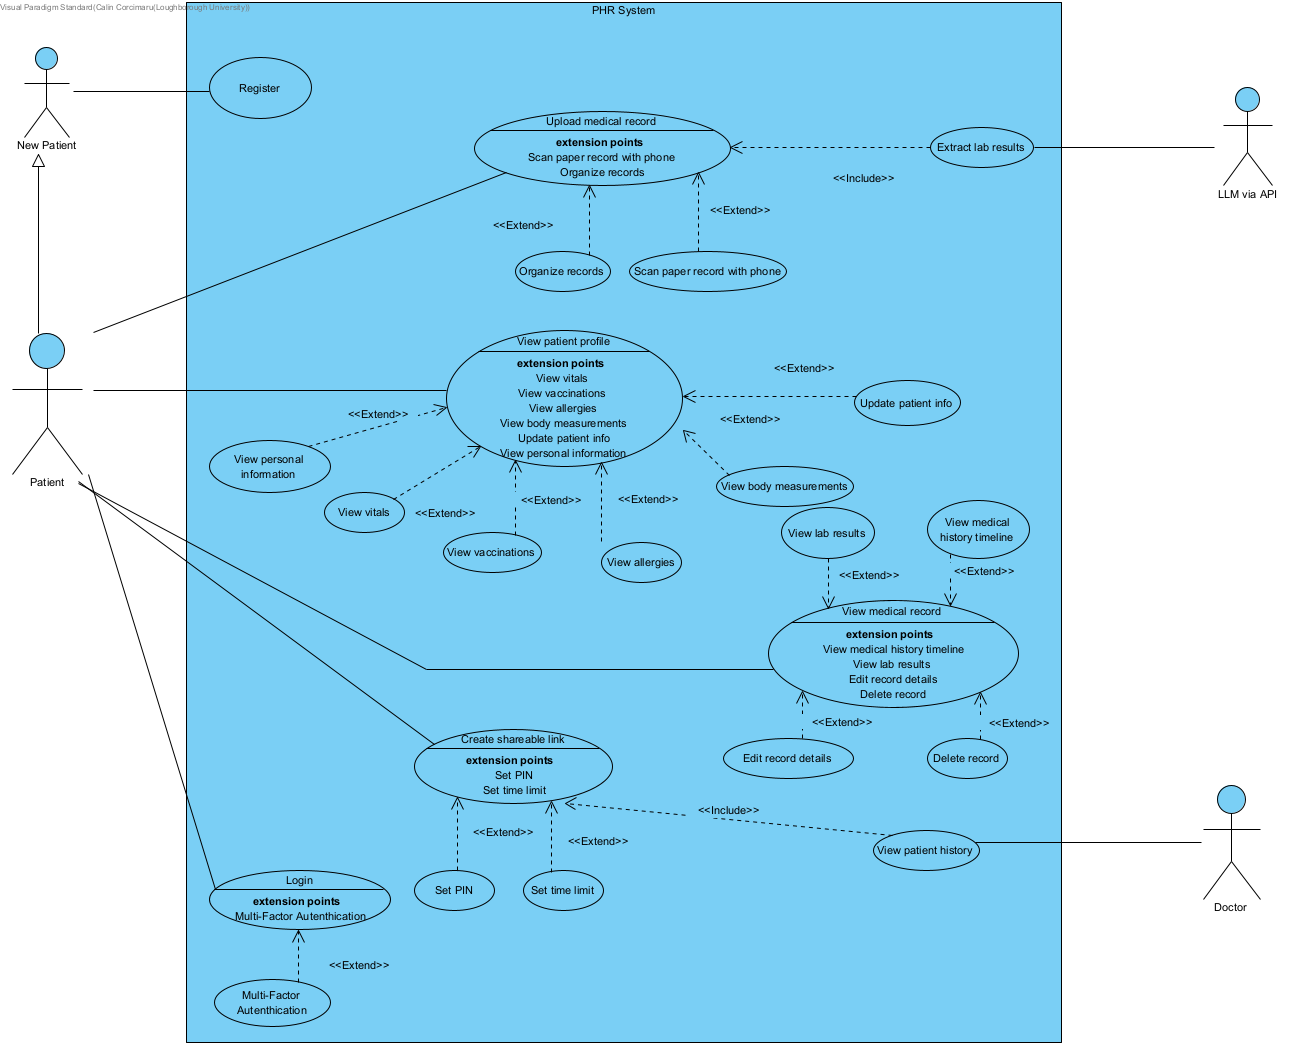
\includegraphics[width=\textwidth]{Use_Case.png}
    \caption{UML Use Case Diagram} 
\end{figure}

\FloatBarrier
\clearpage

\subsubsection{Sequence Diagrams}

\begin{figure}[ht]
    \label{fig:sequence1}
        \centering
        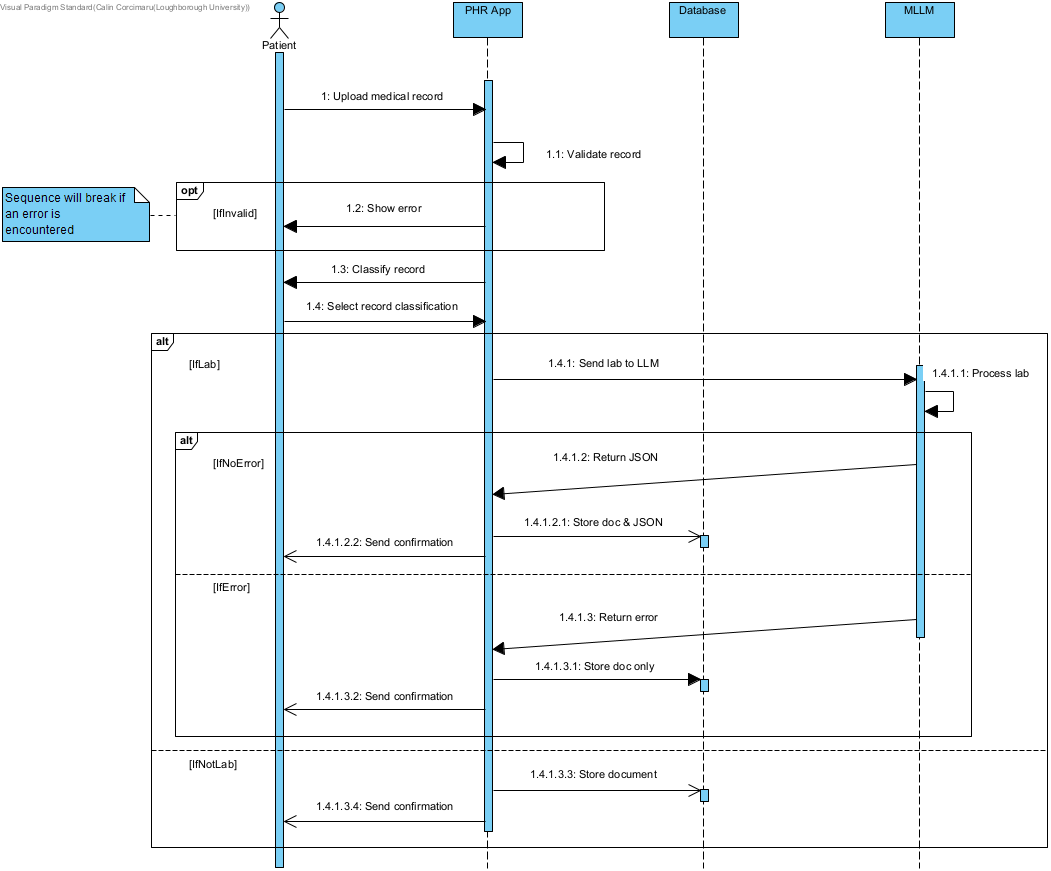
\includegraphics[width=\textwidth]{Sequence_upload.png}
        \caption{UML Sequence Diagram - Upload Record Use Case}
\end{figure}

\begin{figure}[ht]
    \label{fig:sequence2}
        \centering
        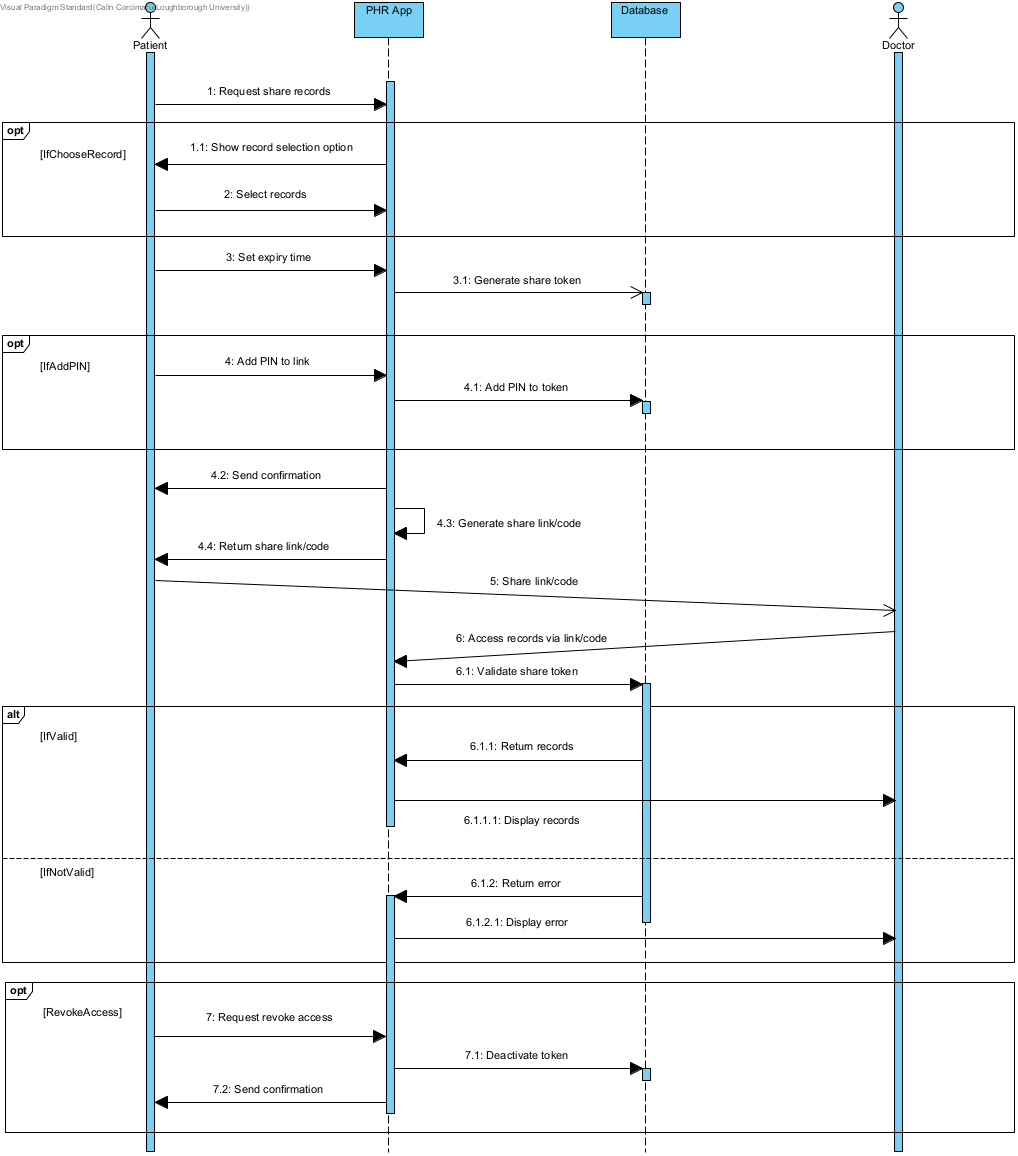
\includegraphics[width=\textwidth]{Sequence_share.png}
        \caption{UML Sequence Diagram - Share Records Use Case}
\end{figure}

\FloatBarrier
\clearpage

\subsubsection{Activity Diagrams}

\begin{figure}[ht]
    \label{fig:activity1}
        \centering
        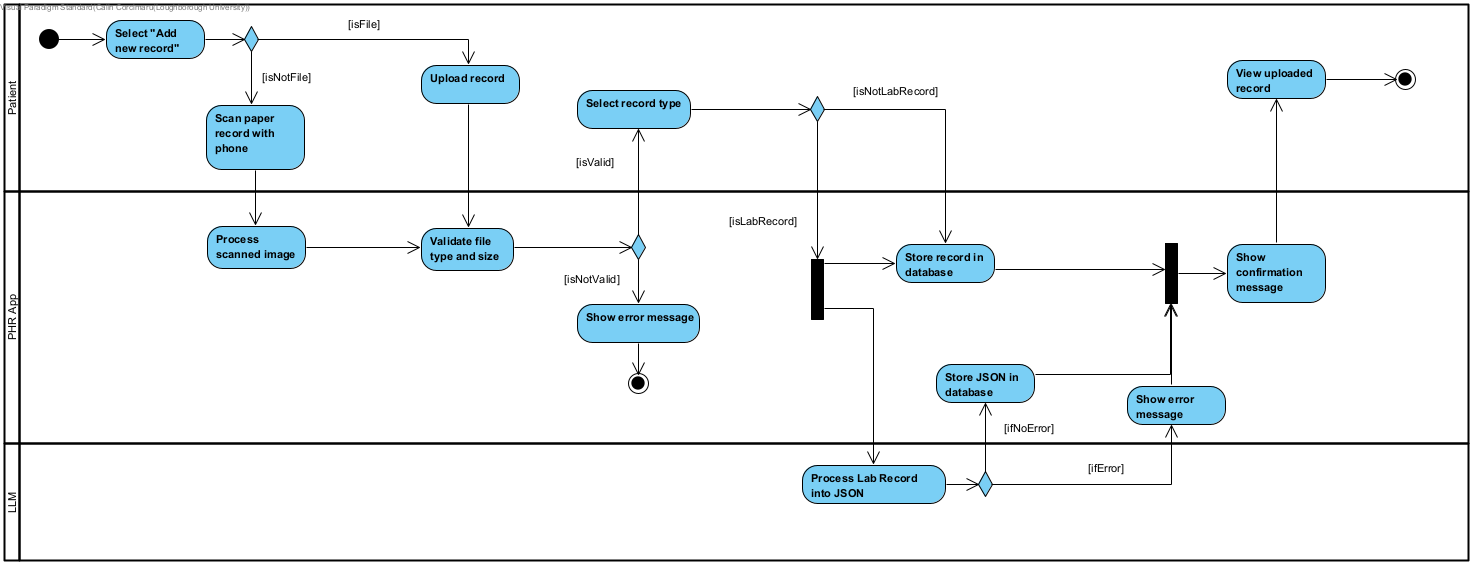
\includegraphics[width=\textwidth]{Activity_upload.png}
        \caption{UML Activity Diagram - Upload Record Use Case}
\end{figure}

\begin{figure}[ht]
    \label{fig:activity2}
        \centering
        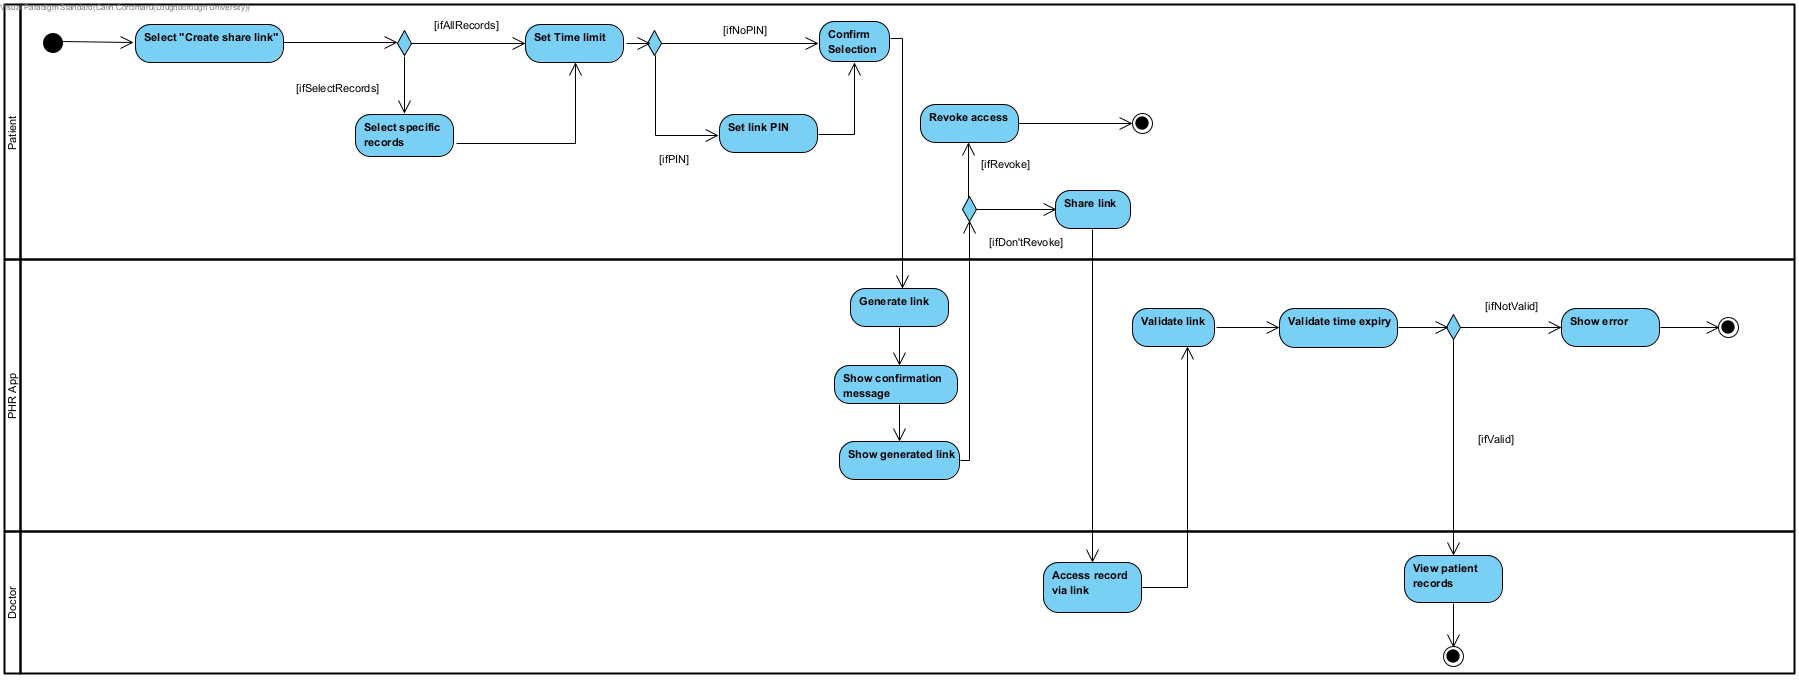
\includegraphics[width=\textwidth]{Activity_link.png}
        \caption{UML Activity Diagram - Share Records Use Case}
\end{figure}

\FloatBarrier
\clearpage

\subsection{Database Design}

\subsection{Wireframes}

\section{Project Tech Stack}

\subsection{Frontend}

\subsection{Backend}

\subsection{Database}

\section{Project Management}

\subsection{Methodology and Tools}

Based on the research above, the student has decided that he will be using a hybrid approach, with Waterfall as the main methodology for planning managing the project. The development part of the project will be done using ScrumBan, so that the student will be able to utilise elements from both frameworks. There are several reasons for this choice:

\begin{enumerate}
    \item The nature of the project - the student is working on a project that has a limited timeframe (about 6-7 months) and is of a smaller scale. 
    \item Documentation requirements - the student is required to document the progress during the project in this report, including the requirements gathered, design considerations and implementation decisions and outcomes. 
    \item Regulatory requirements - the student is required to adhere to the regulations and standards of the healthcare industry, which may require extensive documentation and planning.
    \item Customer involvement - the student will be working closely with the project stakeholder, who will be providing feedback and guidance throughout the project.
    \item Familiarity with both Agile and Waterfall - the student has experience with both Agile (specifically Scrum and Kanban) and Waterfall methodologies, and has worked on projects that have used both approaches.
\end{enumerate}

The student will use Jira Software as their project management tool, which is one of the most popular project management tool for software development projects that supports working with Agile frameworks such as Scrum and Kanban \parencite{atlassian}. The student has experience with Jira Software, having used it in previous projects, and is familiar with its features and capabilities.

\subsection{Project Backlogs}

\subsection{Sprints planning}